
%% bare_conf.tex
%% V1.4a
%% 2014/09/17
%% by Michael Shell
%% See:
%% this can cause conflict
%% http://www.michaelshell.org/
%% for current contact information.
%%
%% This is a skeleton file demonstrating the use of IEEEtran.cls
%% (requires IEEEtran.cls version 1.8a or later) with an IEEE
%% conference paper.
%%
%% Support sites:
%% http://www.michaelshell.org/tex/ieeetran/
%% http://www.ctan.org/tex-archive/macros/latex/contrib/IEEEtran/
%% and
%% http://www.ieee.org/

%%*************************************************************************
%% Legal Notice:
%% This code is offered as-is without any warranty either expressed or
%% implied; without even the implied warranty of MERCHANTABILITY or
%% FITNESS FOR A PARTICULAR PURPOSE! 
%% User assumes all risk.
%% In no event shall IEEE or any contributor to this code be liable for
%% any damages or losses, including, but not limited to, incidental,
%% consequential, or any other damages, resulting from the use or misuse
%% of any information contained here.
%%
%% All comments are the opinions of their respective authors and are not
%% necessarily endorsed by the IEEE.
%%
%% This work is distributed under the LaTeX Project Public License (LPPL)
%% ( http://www.latex-project.org/ ) version 1.3, and may be freely used,
%% distributed and modified. A copy of the LPPL, version 1.3, is included
%% in the base LaTeX documentation of all distributions of LaTeX released
%% 2003/12/01 or later.
%% Retain all contribution notices and credits.
%% ** Modified files should be clearly indicated as such, including  **
%% ** renaming them and changing author support contact information. **
%%
%% File list of work: IEEEtran.cls, IEEEtran_HOWTO.pdf, bare_adv.tex,
%%                    bare_conf.tex, bare_jrnl.tex, bare_conf_compsoc.tex,
%%                    bare_jrnl_compsoc.tex, bare_jrnl_transmag.tex
%%*************************************************************************


% *** Authors should verify (and, if needed, correct) their LaTeX system  ***
% *** with the testflow diagnostic prior to trusting their LaTeX platform ***
% *** with production work. IEEE's font choices and paper sizes can       ***
% *** trigger bugs that do not appear when using other class files.       ***                          ***
% The testflow support page is at:
% http://www.michaelshell.org/tex/testflow/



\documentclass[conference]{IEEEtran}
% Some Computer Society conferences also require the compsoc mode option,
% but others use the standard conference format.
%
% If IEEEtran.cls has not been installed into the LaTeX system files,
% manually specify the path to it like:
% \documentclass[conference]{../sty/IEEEtran}





% Some very useful LaTeX packages include:
% (uncomment the ones you want to load)


% *** MISC UTILITY PACKAGES ***
%
%\usepackage{ifpdf}
% Heiko Oberdiek's ifpdf.sty is very useful if you need conditional
% compilation based on whether the output is pdf or dvi.
% usage:
% \ifpdf
%   % pdf code
% \else
%   % dvi code
% \fi
% The latest version of ifpdf.sty can be obtained from:
% http://www.ctan.org/tex-archive/macros/latex/contrib/oberdiek/
% Also, note that IEEEtran.cls V1.7 and later provides a builtin
% \ifCLASSINFOpdf conditional that works the same way.
% When switching from latex to pdflatex and vice-versa, the compiler may
% have to be run twice to clear warning/error messages.






% *** CITATION PACKAGES ***
%
%\usepackage{cite}
% cite.sty was written by Donald Arseneau
% V1.6 and later of IEEEtran pre-defines the format of the cite.sty package
% \cite{} output to follow that of IEEE. Loading the cite package will
% result in citation numbers being automatically sorted and properly
% "compressed/ranged". e.g., [1], [9], [2], [7], [5], [6] without using
% cite.sty will become [1], [2], [5]--[7], [9] using cite.sty. cite.sty's
% \cite will automatically add leading space, if needed. Use cite.sty's
% noadjust option (cite.sty V3.8 and later) if you want to turn this off
% such as if a citation ever needs to be enclosed in parenthesis.
% cite.sty is already installed on most LaTeX systems. Be sure and use
% version 5.0 (2009-03-20) and later if using hyperref.sty.
% The latest version can be obtained at:
% http://www.ctan.org/tex-archive/macros/latex/contrib/cite/
% The documentation is contained in the cite.sty file itself.






% *** GRAPHICS RELATED PACKAGES ***
%
\ifCLASSINFOpdf
   \usepackage[pdftex]{graphicx}
  % declare the path(s) where your graphic files are
   \graphicspath{{../pdf/}{../jpeg/}}
  % and their extensions so you won't have to specify these with
  % every instance of \includegraphics
   \DeclareGraphicsExtensions{.pdf,.jpeg,.png, .jpg, .gif}
\else
  % or other class option (dvipsone, dvipdf, if not using dvips). graphicx
  % will default to the driver specified in the system graphics.cfg if no
  % driver is specified.
   \usepackage[dvips]{graphicx}
  % declare the path(s) where your graphic files are
   \graphicspath{{../eps/}}
  % and their extensions so you won't have to specify these with
  % every instance of \includegraphics
   \DeclareGraphicsExtensions{.eps}
\fi
% graphicx was written by David Carlisle and Sebastian Rahtz. It is
% required if you want graphics, photos, etc. graphicx.sty is already
% installed on most LaTeX systems. The latest version and documentation
% can be obtained at: 
% http://www.ctan.org/tex-archive/macros/latex/required/graphics/
% Another good source of documentation is "Using Imported Graphics in
% LaTeX2e" by Keith Reckdahl which can be found at:
% http://www.ctan.org/tex-archive/info/epslatex/
%
% latex, and pdflatex in dvi mode, support graphics in encapsulated
% postscript (.eps) format. pdflatex in pdf mode supports graphics
% in .pdf, .jpeg, .png and .mps (metapost) formats. Users should ensure
% that all non-photo figures use a vector format (.eps, .pdf, .mps) and
% not a bitmapped formats (.jpeg, .png). IEEE frowns on bitmapped formats
% which can result in "jaggedy"/blurry rendering of lines and letters as
% well as large increases in file sizes.
%
% You can find documentation about the pdfTeX application at:
% http://www.tug.org/applications/pdftex





% *** MATH PACKAGES ***
%
%\usepackage[cmex10]{amsmath}
% A popular package from the American Mathematical Society that provides
% many useful and powerful commands for dealing with mathematics. If using
% it, be sure to load this package with the cmex10 option to ensure that
% only type 1 fonts will utilized at all point sizes. Without this option,
% it is possible that some math symbols, particularly those within
% footnotes, will be rendered in bitmap form which will result in a
% document that can not be IEEE Xplore compliant!
%
% Also, note that the amsmath package sets \interdisplaylinepenalty to 10000
% thus preventing page breaks from occurring within multiline equations. Use:
%\interdisplaylinepenalty=2500
% after loading amsmath to restore such page breaks as IEEEtran.cls normally
% does. amsmath.sty is already installed on most LaTeX systems. The latest
% version and documentation can be obtained at:
% http://www.ctan.org/tex-archive/macros/latex/required/amslatex/math/





% *** SPECIALIZED LIST PACKAGES ***
%
%\usepackage{algorithmic}
% algorithmic.sty was written by Peter Williams and Rogerio Brito.
% This package provides an algorithmic environment fo describing algorithms.
% You can use the algorithmic environment in-text or within a figure
% environment to provide for a floating algorithm. Do NOT use the algorithm
% floating environment provided by algorithm.sty (by the same authors) or
% algorithm2e.sty (by Christophe Fiorio) as IEEE does not use dedicated
% algorithm float types and packages that provide these will not provide
% correct IEEE style captions. The latest version and documentation of
% algorithmic.sty can be obtained at:
% http://www.ctan.org/tex-archive/macros/latex/contrib/algorithms/
% There is also a support site at:
% http://algorithms.berlios.de/index.html
% Also of interest may be the (relatively newer and more customizable)
% algorithmicx.sty package by Szasz Janos:
% http://www.ctan.org/tex-archive/macros/latex/contrib/algorithmicx/




% *** ALIGNMENT PACKAGES ***
%
%\usepackage{array}
% Frank Mittelbach's and David Carlisle's array.sty patches and improves
% the standard LaTeX2e array and tabular environments to provide better
% appearance and additional user controls. As the default LaTeX2e table
% generation code is lacking to the point of almost being broken with
% respect to the quality of the end results, all users are strongly
% advised to use an enhanced (at the very least that provided by array.sty)
% set of table tools. array.sty is already installed on most systems. The
% latest version and documentation can be obtained at:
% http://www.ctan.org/tex-archive/macros/latex/required/tools/


% IEEEtran contains the IEEEeqnarray family of commands that can be used to
% generate multiline equations as well as matrices, tables, etc., of high
% quality.




% *** SUBFIGURE PACKAGES ***
%\ifCLASSOPTIONcompsoc
%  \usepackage[caption=false,font=normalsize,labelfont=sf,textfont=sf]{subfig}
%\else
%  \usepackage[caption=false,font=footnotesize]{subfig}
%\fi
% subfig.sty, written by Steven Douglas Cochran, is the modern replacement
% for subfigure.sty, the latter of which is no longer maintained and is
% incompatible with some LaTeX packages including fixltx2e. However,
% subfig.sty requires and automatically loads Axel Sommerfeldt's caption.sty
% which will override IEEEtran.cls' handling of captions and this will result
% in non-IEEE style figure/table captions. To prevent this problem, be sure
% and invoke subfig.sty's "caption=false" package option (available since
% subfig.sty version 1.3, 2005/06/28) as this is will preserve IEEEtran.cls
% handling of captions.
% Note that the Computer Society format requires a larger sans serif font
% than the serif footnote size font used in traditional IEEE formatting
% and thus the need to invoke different subfig.sty package options depending
% on whether compsoc mode has been enabled.
%
% The latest version and documentation of subfig.sty can be obtained at:
% http://www.ctan.org/tex-archive/macros/latex/contrib/subfig/




% *** FLOAT PACKAGES ***
%
%\usepackage{fixltx2e}
% fixltx2e, the successor to the earlier fix2col.sty, was written by
% Frank Mittelbach and David Carlisle. This package corrects a few problems
% in the LaTeX2e kernel, the most notable of which is that in current
% LaTeX2e releases, the ordering of single and double column floats is not
% guaranteed to be preserved. Thus, an unpatched LaTeX2e can allow a
% single column figure to be placed prior to an earlier double column
% figure. The latest version and documentation can be found at:
% http://www.ctan.org/tex-archive/macros/latex/base/


%\usepackage{stfloats}
% stfloats.sty was written by Sigitas Tolusis. This package gives LaTeX2e
% the ability to do double column floats at the bottom of the page as well
% as the top. (e.g., "\begin{figure*}[!b]" is not normally possible in
% LaTeX2e). It also provides a command:
%\fnbelowfloat
% to enable the placement of footnotes below bottom floats (the standard
% LaTeX2e kernel puts them above bottom floats). This is an invasive package
% which rewrites many portions of the LaTeX2e float routines. It may not work
% with other packages that modify the LaTeX2e float routines. The latest
% version and documentation can be obtained at:
% http://www.ctan.org/tex-archive/macros/latex/contrib/sttools/
% Do not use the stfloats baselinefloat ability as IEEE does not allow
% \baselineskip to stretch. Authors submitting work to the IEEE should note
% that IEEE rarely uses double column equations and that authors should try
% to avoid such use. Do not be tempted to use the cuted.sty or midfloat.sty
% packages (also by Sigitas Tolusis) as IEEE does not format its papers in
% such ways.
% Do not attempt to use stfloats with fixltx2e as they are incompatible.
% Instead, use Morten Hogholm'a dblfloatfix which combines the features
% of both fixltx2e and stfloats:
%
% \usepackage{dblfloatfix}
% The latest version can be found at:
% http://www.ctan.org/tex-archive/macros/latex/contrib/dblfloatfix/




% *** PDF, URL AND HYPERLINK PACKAGES ***
%
%\usepackage{url}
% url.sty was written by Donald Arseneau. It provides better support for
% handling and breaking URLs. url.sty is already installed on most LaTeX
% systems. The latest version and documentation can be obtained at:
% http://www.ctan.org/tex-archive/macros/latex/contrib/url/
% Basically, \url{my_url_here}.




% *** Do not adjust lengths that control margins, column widths, etc. ***
% *** Do not use packages that alter fonts (such as pslatex).         ***
% There should be no need to do such things with IEEEtran.cls V1.6 and later.
% (Unless specifically asked to do so by the journal or conference you plan
% to submit to, of course. )


% correct bad hyphenation here
\hyphenation{optical networks semiconductor}


\begin{document}
%
% paper title
% Titles are generally capitalized except for words such as a, an, and, as,
% at, but, by, for, in, nor, of, on, or, the, to and up, which are usually
% not capitalized unless they are the first or last word of the title.
% Linebreaks \\ can be used within to get better formatting as desired.
% Do not put math or special symbols in the title.
\title{Analyzing performance of A* and Bidirectional Bearch on well-defined problems}

% author names and affiliations
% use a multiple column layout for up to three different
% affiliations
\author{\IEEEauthorblockN{Bat-Orgil Batsaikhan}
\IEEEauthorblockA{CSCI4511W - Intro to Artificial Intelligence\\
University of Minnesota, Twin-Cities\\
Email: batsa003@umn.edu}
}

% make the title area
\maketitle

% As a general rule, do not put math, special symbols or citations
% in the abstract
\begin{abstract}
In this paper, I have analyzed and compared an A* search and a Bidirectional Search on the Tower of Hanoi and the Fifteen puzzle. This paper explores the time and memory differences of these two algorithms. The experiment consisted of test scenarios with increasing difficulty of the puzzles. As a result of the experiment, the A* search outperforms several times better than the bidirectional search on both of the puzzles. In addition, the bottleneck of these algorithms was memory usage, as the puzzles get bigger.
\end{abstract}

% no keywords


% For peer review papers, you can put extra information on the cover
% page as needed:
% \ifCLASSOPTIONpeerreview
% \begin{center} \bfseries EDICS Category: 3-BBND \end{center}
% \fi
%
% For peerreview papers, this IEEEtran command inserts a page break and
% creates the second title. It will be ignored for other modes.
\IEEEpeerreviewmaketitle

\section{Introduction}

% no \IEEEPARstart
% You must have at least 2 lines in the paragraph with the drop letter
% (should never be an issue)

It is of a great interest to compare a heuristic search algorithms to a classical search algorithms. In a search problem, we are given a simple directed graph and the initial state. The objective of the search is to find a path to the goal state that satisfies certain conditions. The main goal of the heuristic algorithms is to make choices so that the bad paths don't have to be explored, thus saving time and memory. This technique is an interesting challenge in Artificial Intelligence due to the difficulty of theoretical and experimental analysis of these in comparison with other classical algorithms, and the concept of heuristic or guessing underlie the whole field of Artificial Intelligence. On the other hand, classical search algorithms work for any general graph, don't use any specific properties and characteristics of the graph, and therefore is non-heuristic. In this paper, I have analyzed and compared the A* heuristic search and the Bidirectional BFS. The objective of this experiment is to give an insight on efficiency, implementation, and limitations of A* search algorithm and the classical the Bidirectional Search.

Both of the algorithms are popular and known for their efficiency. The A* algorithm is a heuristic graph-searching algorithm and is most widely known form of Best-First Search. It was introduced around 1960's for finding shortest paths. Since that time, it has been applied successfully in many domains such as game AI, robotics, and graphs. On the other hand, the Bidirectional search is known for cutting the exponent of the complexity; thus, significantly improves the efficiency compared to simple search.

In recent years, many applications and variations of the A* search is developed. For example, it is used for GPS applications for providing shortest path. Given a map, finding shortest distance between two given locations is difficult because there are many intermediate locations, places, and roads. With a heuristic knowledge that the optimal path somewhat looks like a straight line between these locations, the A* search uses heuristic function to search through nodes that seem to lie on a straight line from source to destination.

The Bidirectional search is known for its robustness for finding shortest distance between two nodes. Unlike the A* search, which is a unidirectional algorithm, the Bidirectional search takes advantage of the known goal nodes by searching backward from the goal node. Efficient use of memory crucial for the bidirectional search algorithm's performance because the two search from both nodes will have to meet at some point, and they have to keep track of the nodes visited and actions taken from the previous node, doubling the space of two unidirectional search.

In this experiment, we will focus on finding the complete solution of the puzzle. Kaindl and Khorsand constructed very efficient memory-bounded bidirectional search that could be used for finding near-optimal solutions. They also showed that bidirectional approach rather than the unidirectional approach is better. \cite{KandKh} However, in this paper, we will only consider the problem of finding the complete solution of the puzzles because it could be very complex task to define the "closeness" to the goal state and doing analysis on it.

\begin{figure}[!t]
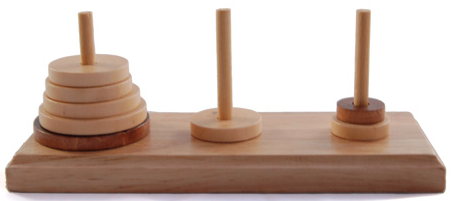
\includegraphics[width=8cm, height=4cm]{towerofhanoi}
\centering
\caption{Initial state of the Tower of Hanoi with 3 pegs and 5 disks.}
%\label{fig_sim}
\end{figure}

The Tower of Hanoi consists of a number of pegs and a number of disks with different sizes. In this experiment, we only consider a Tower of Hanoi with 3 pegs. Initially, all of the disks are on the first peg in ascending order of size, the largest at the bottom. The objective of the puzzle is to move all of the disks into the last peg. At each turn, we can pick up upper disk from one of the peg and placing it on top of another peg, and the disk we picked must be smaller than the top disk of the destination stack (unless the destination stack is empty). Figure 1 shows an example of the Tower of Hanoi.

The sliding puzzle is a general term used for a type of puzzles where the player is allowed to slide pieces along path. In the experiment, we consider the Fifteen Puzzle or 4 by 4 sliding puzzle. We start from a random shuffled numbers from one to fifteen in 4 by 4 grid where one of the tile is missing. The objective of the puzzle is to place the tiles in order by moving the missing tile horizontally or vertically. Figure 2 shows an example of completely solved Fifteen Puzzle.

The Tower of Hanoi and the Fifteen Puzzle are great fit for the Bidirectional Search, since the goal states in these puzzle are completely determined. We can reverse the any move from these puzzle, which allows the Bidirectional search to to traverse backwards from the goal state. The Bidirectional search takes advantage of the known goal state by searching from both start and end states. In my experiments, I have used Breadth First Search from both ends, where the algorithm stops when two searches meet. Breadth first search (BFS) is mostly used in the Bidirectional Search since bfs explores the neighbors first, then second neighbors, and so on. In these puzzles, this means that we're exploring states that are one moves away, two moves away, and so on. Two BFS from both ends will be guaranteed to intersect after exploring nodes that are $\frac{d}{2}$ edges away. On the other hand, A* search is a unidirectional algorithm where the end state is not not necessarily given. It only keeps track of the states that are visited along the search.

These puzzles can be extended into different puzzles, and they have many practical applications. For example, the sliding puzzle has many variations including word puzzle, 7 by 7 sliding block, and Klotski puzzle. The Tower of Hanoi has been a great interest to researchers because of its abstraction and difficulty. It also frequently used in psychological research on problem solving.

\begin{figure}[!t]
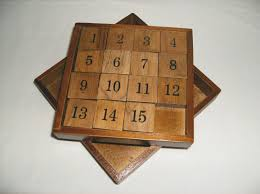
\includegraphics[width=8cm, height=4cm]{slidingpuzzle}
\centering
\caption{Completely solved fifteen puzzle}
%\label{fig_sim}
\end{figure}

The A* search is known to be one of the most suitable and efficient algorithm among heuristic path-finding algorithms such as Hill Climbing, Steepest-ascent, Best-First, and A* search algorithms. \cite{Potdar}

Given the nature of the A* search, these problems have interesting challenges of coming up with a good heuristic functions to make A* work. Specifically for the Tower of Hanoi, not many experiments are done using the A* search or any evaluation of the heuristics. Korf showed that the current heuristic search algorithms has high computational costs and lack real-time application in puzzles, including the sliding puzzle. \cite{Korf}

My experiments on various test cases of the Tower of Hanoi and the Fifteen Puzzle shows that the A* search outperforms bidirectional both in time and space. In the Tower of Hanoi, even though the memory usage/nodes generated was was similar, A* was faster than the Bidirectional Search.

%\hfill mds
%\hfill September 17, 2014

%\subsection{Memory comparison of the algorithms known}
%Subsection text here. blabl blalbalba $O(2^N)$ hehe


%\subsubsection{Time complexity comparison of these algorithms}
%Just put stuff about TIME complexity. Just put a lot of stuff here. \cite{Prince04}

% An example of a floating figure using the graphicx package.
% Note that \label must occur AFTER (or within) \caption.
% For figures, \caption should occur after the \includegraphics.
% Note that IEEEtran v1.7 and later has special internal code that
% is designed to preserve the operation of \label within \caption
% even when the captionsoff option is in effect. However, because
% of issues like this, it may be the safest practice to put all your
% \label just after \caption rather than within \caption{}.
%
% Reminder: the "draftcls" or "draftclsnofoot", not "draft", class
% option should be used if it is desired that the figures are to be
% displayed while in draft mode.
%


% Note that IEEE typically puts floats only at the top, even when this
% results in a large percentage of a column being occupied by floats.


% An example of a double column floating figure using two subfigures.
% (The subfig.sty package must be loaded for this to work.)
% The subfigure \label commands are set within each subfloat command,
% and the \label for the overall figure must come after \caption.
% \hfil is used as a separator to get equal spacing.
% Watch out that the combined width of all the subfigures on a 
% line do not exceed the text width or a line break will occur.
%
%\begin{figure*}[!t]
%\centering
%\subfloat[Case I]{\includegraphics[width=2.5in]{box}%
%\label{fig_first_case}}
%\hfil
%\subfloat[Case II]{\includegraphics[width=2.5in]{box}%
%\label{fig_second_case}}
%\caption{Simulation results for the network.}
%\label{fig_sim}
%\end{figure*}
%
% Note that often IEEE papers with subfigures do not employ subfigure
% captions (using the optional argument to \\subfloat[]), but instead will
% reference/describe all of them (a), (b), etc., within the main caption.
% Be aware that for subfig.sty to generate the (a), (b), etc., subfigure
% labels, the optional argument to \\subfloat must be present. If a
% subcaption is not desired, just leave its contents blank,
% e.g., \\subfloat[].

% \begin{equation}
%  \sum_{i=1}^{\infty} \frac{1}{n^s} 
% \end{equation}

% An example of a floating table. Note that, for IEEE style tables, the
% \caption command should come BEFORE the table and, given that table
% captions serve much like titles, are usually capitalized except for words
% such as a, an, and, as, at, but, by, for, in, nor, of, on, or, the, to
% and up, which are usually not capitalized unless they are the first or
% last word of the caption. Table text will default to \footnotesize as
% IEEE normally uses this smaller font for tables.
% The \label must come after \caption as always.
%
%\begin{table}[!t]
%% increase table row spacing, adjust to taste
%\renewcommand{\arraystretch}{1.3}
% if using array.sty, it might be a good idea to tweak the value of
% \extrarowheight as needed to properly center the text within the cells
%\caption{An Example of a Table}
%\label{table_example}
%\centering
%% Some packages, such as MDW tools, offer better commands for making tables
%% than the plain LaTeX2e tabular which is used here.
%\begin{tabular}{|c||c|}
%\hline
%One & Two\\
%\hline
%Three & Four\\
%\hline
%\end{tabular}
%\end{table}


% Note that the IEEE does not put floats in the very first column
% - or typically anywhere on the first page for that matter. Also,
% in-text middle ("here") positioning is typically not used, but it
% is allowed and encouraged for Computer Society conferences (but
% not Computer Society journals). Most IEEE journals/conferences use
% top floats exclusively. 
% Note that, LaTeX2e, unlike IEEE journals/conferences, places
% footnotes above bottom floats. This can be corrected via the
% \fnbelowfloat command of the stfloats package.


\section{Experiment Methods}

\begin{figure}[!t]
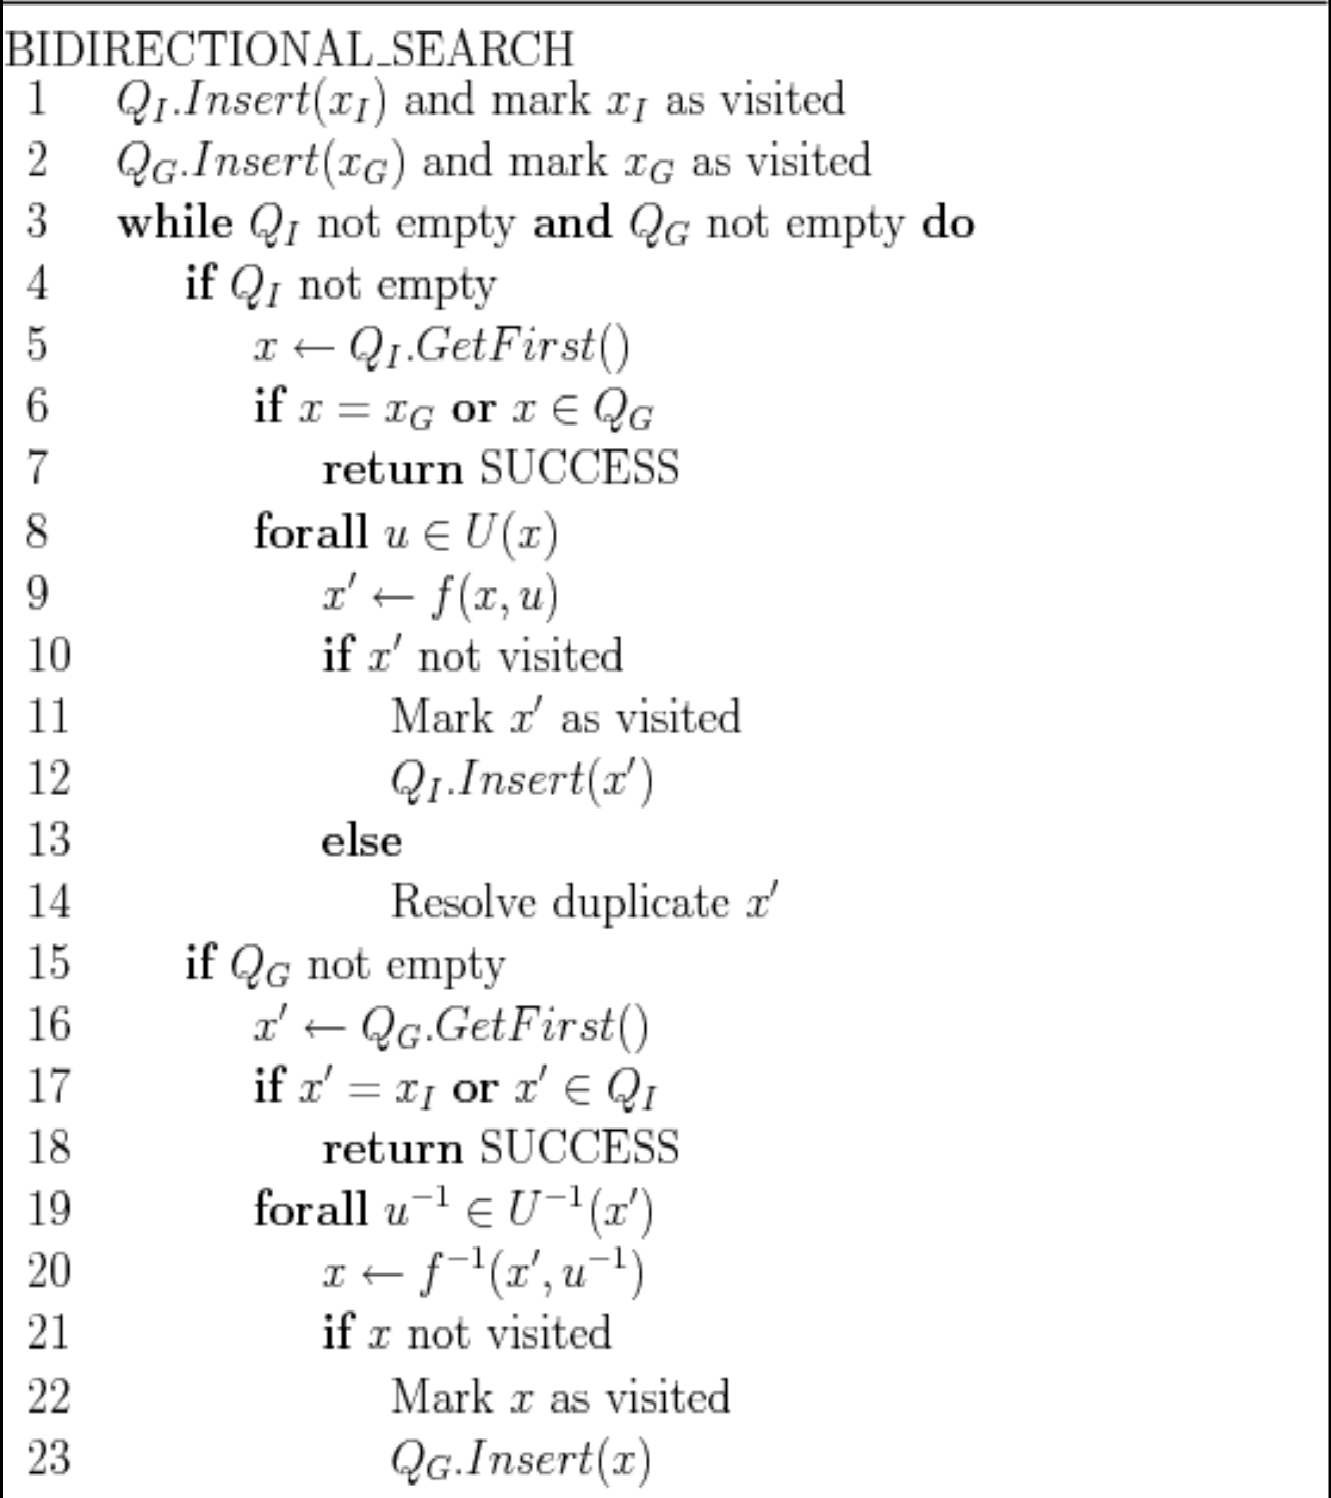
\includegraphics[width=8cm, height=8cm]{BI_Pseudocode}
\centering
\caption{Bidirectional Search Algorithm}
%\label{fig_sim}
\end{figure}

Since the graphs that are created from the are too large to store explicitly, it is more reasonable to discuss the theoretical analysis based on the branching factor and the solution depth. Branching factor is simply the number of children expanding from a node, and the solution depth is the number of edges on the solution path between the start and the end states.

The Bidirectional search pseudo-code is shown in the Figure 3. It is essentially two breadth first search from both start state $x_I$ and goal state $x_G$. $Q_I$ and $Q_G$ represents queues that are used by initial state and goal state respectively. We pop a node from the queue one at a time alternating between two queues, and push all of its neighbors who is not visited before. Therefore, the Bidirectional Search will be balanced from both start and end state, and this is important for theoretical time complexity of the algorithm. Note that $f^{-1}$ and $U^{-1}$ corresponds to inverse of the function that applies given action to a state and the list of actions respectively.

To mark a given state as a visited, we hash the state into a 64 bit long integer. There are at most 16 disks/cells in both puzzles; therefore, we could simply use 4 bits to represent each cell's position among 16 cells. In the Tower of Hanoi, it is sufficient to hash each peg since there are only 3 of them, and each peg is simply at most 16 numbers where each number could be represented by 4 bits. For the Fifteen Puzzle, for each of its 16 position, we simply represent the number that the cell is containing in 4 bits (since numbers are 0-15). This implementation of hashing provides efficient lookup for marking the state to be visited.

In the Tower of Hanoi, it is known that solving initial state with $n$ disks requires $2^n - 1$ moves to reach the end state. To find the branching factor, let's consider the only disks on top of the stacks. Since we are only allowed to move smaller disk on top of a bigger disk, among 6 possible movement, half of them are legal. This leaves us with 3 possible moves. However, one of these moves will take it to the previous state; therefore, we have a 2 moves to consider. Therefore, in the Tower of Hanoi, branching factor $b = 2$ while shallowest depth of the solution $d = 2^n - 1$. In my experiment, we simply tested it on $n = 1$ to $n = 16$, incremented by 1 at a time.

In the Fifteen Puzzle, we have four directions to move the tile number 0 (empty tile), and one of these four moves will be a reverse move of the previous state. Therefore, there are three possible children of this node, and the branching factor is $b = 3$. The shallowest depth is the minimum number of moves required to solve the puzzle. In my experiment, this number of moves was varied starting from $d = 18$ to $d = 50$, incrementing by 4.

The Bidirectional search has a time complexity $O(b^{d/2})$ and space complexity $O(b^{d/2})$ where $b$ is a branching factor while $d$ is the shallowest depth of the solution. This is because two breadth first searches will intersect when they have explored nodes that are $d/2$ away. Since, the both time and space complexity for breadth first search is $O(b^d)$, the Bidirectional search has complexity $O(b^{d/2})$. 


\begin{figure}[!t]
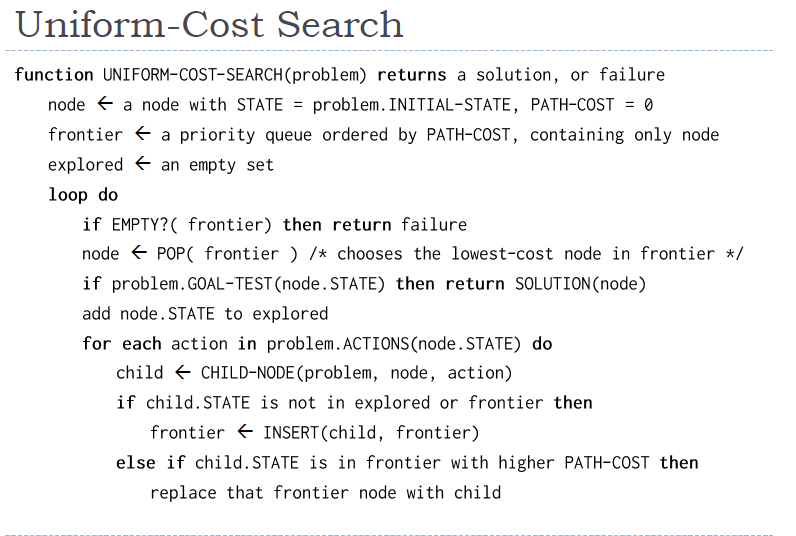
\includegraphics[width=8cm]{uniform_cost}
\centering
\caption{Uniform-Cost Search Algorithm}
%\label{fig_sim}
\end{figure}

The A* Search is the informed version of Uniform Cost Search. It differs in that you have to will make informed decisions on which point to expand by approximating how close it is to the goal state. Uniform cost search is guided by path cost rather than a depth, and the worst case time complexity is $O(b^{C^*/e})$ where $C*$ is the cost of the optimal solution and assuming that every action costs at least $e$. In this experiment, all of the steps are equal; therefore, the worst case time complexity is $O(b^{d+1})$.

In the pseudo-code provided on Figure 4, inside of the main loop, we need to pop a node from the frontier using $POP(frontier)$ method. In uniform-cost search, we pop a node with the smallest path-cost. It determines which node to expand based on the $f(x)$ function which is an approximate total cost at node $x$. The A* uses two supplementary cost functions to determine $f(x)$.

$g(x)$: The real cost to reach node x. It is determined by sum of edge weights along the path from the start state to $x$.

$h(x)$: It is an approximate cost from node $x$ to the goal state, which is a heuristic function.

Then, the total cost at node $x$ is given by

\begin{equation}
    f(x) = g(x) + h(x)
\end{equation}

At each iteration of the loop, we will expand a node that $x$ has the least $f(x)$ from the frontier queue. While considering its neighbors, we also have extra condition to make sure that we only add nodes with higher $f$.

Even though the A* search has a worst case time complexity of $O(b^d)$, the heuristics of the A* greatly affects the time and space usage. For constant step costs, it is known to be $O(b^{ed})$ where $d$ is the depth of a solution and $e$ is a relative error defined by the difference of cost of getting from root to the goal and $h$.

The A* heuristic function for the Tower of Hanoi was simply number of disks not in the final position at any given state. Intuitively, the more discs we move to the final peg, the closer it is getting to the state. Even though it is not a perfect heuristic, it will help us to explore nodes that seems closer to the goal state.

For sliding puzzle, the heuristic function of the A* was sum of all Manhattan distance between each cell's current position and its goal state position. The Manhattan distance for a certain cell to its destined position indicates how many moves are needed to move this cell to its destined position in least number of moves. When each of the cell gets closer to its destined position, it is good indication of approaching the solution. 

According to the big O time and space complexity, the Bidirectional Search has better worst case complexity; therefore, it is reasonable to expect the Bidirectional Search to be more efficient than the A*. However, this doesn't mean that the A* would be slow because we don't know how much improvement does the heuristic function will make compared to the worst case scenario. 

\section{Experimental results and Analysis}

My experimental result consists of two parts where we analyzed both algorithms on each of the problems, and for each problem I compared the time it takes to solve the puzzle and the number of nodes generated/explored in order to solve the puzzle.

\subsection{Experimental result for the Tower of Hanoi}

\begin{figure}[!t]
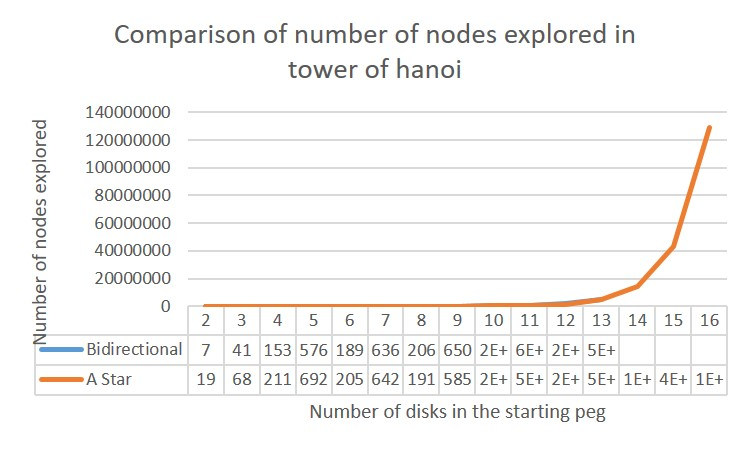
\includegraphics[width=8cm]{hanoiNodes}
\centering
\caption{Comparison of number of nodes explored in the Tower of Hanoi (Note that both algorithms generated approximately same number of nodes when the number of disks is less than or equal to 13. However, the Bidirectional Search didn't successfully terminate under constraint when $n$ = 14)}
\label{fig_sim}
\end{figure}

\begin{figure}[!t]
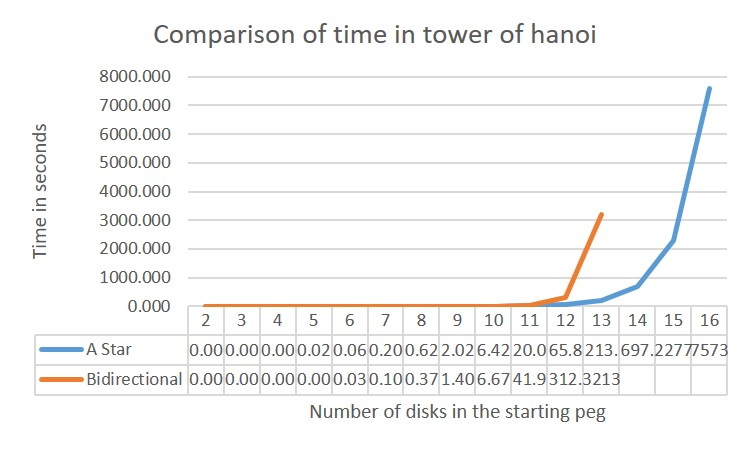
\includegraphics[width=8cm]{hanoiTime}
\centering
\caption{Comparison of time it takes to complete the Tower of Hanoi}
\label{fig_sim}
\end{figure}

The initial state of the Tower of Hanoi only depends on the number of disks $n$, and these $n$ disks are piled from smallest to largest (largest on the bottom). I ran my experiments on both algorithms until we run out space or if it runs more than several hours.

In the Bidirectional search, the cut-off point was when the program memory usage was more than 30GB where it wasn't able to continue program execution. The search memory usage exceeded 30GB when $n = 14$.

In the A* search, the cut-off point was when the program ran more than 6 hours. It was uncertain when the program would finish, and this scenario occurs when $n = 17$. 

From Figure 5, we can see that both algorithms generated/explored approximately same number of nodes. 
The graph from figure 4 indicates that the A* search was more efficient in terms of time it takes to complete. Specifically, when $n$ starts to get bigger, the A* search was consistent while the Bidirectional search slowed down much more dramatically once $n = 14$. 

\subsection{Experimental result for the Fifteen puzzle}

The initial states of the puzzle are initially $d$ moves away from the goal state. And in the experiment, I varied $d$ from $18$ to $50$ with increasing $d$ by 4 at a time.

For both of the algorithms, the cut-off point of the program was the program memory usage exceeded 30GB where it wasn't able to continue program execution. This occurred for the Bidirectional search when the number of moves $d = 46$. In the A* search, the cut-off point was $d = 50$. 

Figure 5 indicates that the Bidirectional Search explored approximately 5 times more nodes than the A* search. Figure 6 indicates that the A* search was more efficient in terms of time it takes to complete, and it was able to finish $d = 46$ puzzle within the time and memory constraint.

\begin{figure}[!t]
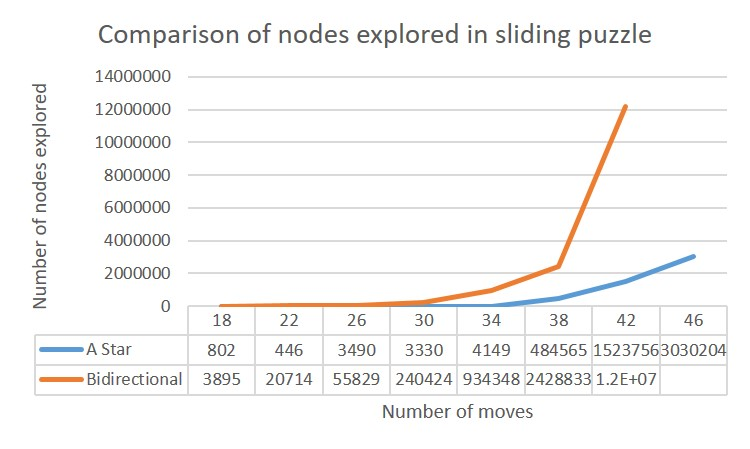
\includegraphics[width=8cm]{slidingNodes}
\centering
\caption{Comparison of number of nodes explored in sliding puzzle tests}
\label{fig_sim}
\end{figure}

\begin{figure}[!t]
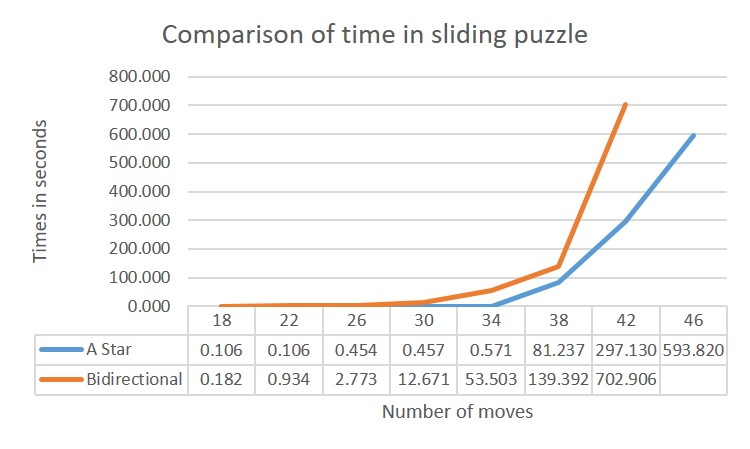
\includegraphics[width=8cm]{slidingTime}
\centering
\caption{Comparison of time it takes to complete the sliding puzzle tests}
\label{fig_sim}
\end{figure}

\subsection{Analysis of the result}

The experiment shows that the A* search outperforms the Bidirectional search in most of the scenarios in terms of both time and space.

There could be several factors that are influencing the performance of the Bidirectional Search. In the Bidirectional search, we are cutting the depth in half; however, this also means that we have a doubled the space in terms of keeping track of nodes. Also, the hash function for the Bidirectional Search has to be fast enough. We are iterating through the state with at most 16 entries for both problems; therefore, the time complexity will have a big constant factor in terms of hashing and storing the visited nodes. In general, since we are using more node in the Bidirectional Search, it will slow down the program in terms of both memory and time.

It is very difficult to theoretically explain the superior performance of the A* search compared to the Bidirectional search. As we can see, even though the worst case complexity of the A* is asymptotically lower than the Bidirectional Search, the heuristic function plays important role for the performance of the A*. Specifically in the Fifteen puzzle, we can see the efficiency clearly both in terms of time and space. It suggests that, when it comes to solving these problems correctly, the intuition of choosing the right nodes to explore is important. Even with simple heuristics, it was able to perform well due to the nature of the problem where it is possible to waste a lot of time and space by taken a wrong action and exploring wrong subtrees. The A*, in general, was able to steer the exploration in the right direction. 
Both of the algorithm ran out of memory first because they both need to keep track of the visited nodes. In the A* search we have the nodes in the priority queue and pops one at a time, while the Bidirectional Search also keeps track of two queues that are used for BFS which stores all of the nodes to be visited.

In terms of time of execution, the A* algorithm is faster than the Bidirectional Search several times. On the other hand, in terms of memory usage, the A* algorithm is still slightly more efficient due to fewer number of nodes explored. Also, the A* algorithm was scalable up to $d = 17$ for the Tower of Hanoi and $d = 46$ for the Fifteen Puzzle. Therefore, to summarize, the A* search was faster, memory efficient, and more scalable compared to the Bidirectional Search.

From these experiments, we can observe the general tendency that the A* is faster than the Bidirectional search by factor of three to four, specifically when the problem size gets bigger. For smaller values, we can't tell much difference. However, it is unpredictable how it would scale in bigger numbers; therefore, numerical estimation is difficult. Since the number of nodes explored is also a way to compare memory usage, the graph shows that the A* search used less memory due to its efficient exploration. It can be explained by how the Bidirectional Search blindly explores neighbors while the A* search was smart when it comes to choosing which node to explore.

\section{Conclusion and Future Work}
In my experiment, the A* search outperformed the Bidirectional search both in terms of time space. Regardless of worst case time complexity of these algorithms, the A* algorithm was able to explore less nodes in process of solving the puzzle. The reason of efficiency in the A* search could be coming from its intuitive and efficient choice of node expansion. The nature of the Tower of Hanoi and the Fifteen puzzle are such that the even with general guideline due to small heuristics can significantly improve the efficiency.

The worst case complexity of the A* search was much slower than that of the Bidirectional Search. Regardless, the A* search was several time efficient. Therefore, it is reasonable to more carefully analyze the complexity of the A* search using effective branching factors or more higher level analysis techniques.

Both of these algorithms need to be implemented carefully in terms of memory usage. Because we have to keep track of all visited nodes, it consumes the most memory and slows down the execution of the program. The time was not the limitation for both of these algorithms. It is unknown how much the algorithms will improve if we try different data structures and ways of storing the nodes, data, and the puzzle. We could explore is efficient use of data structures in the program. Memory usage was one of the bottleneck of these algorithms, and the Bidirectional Search wasn't even able to run more due to its memory constraint. Therefore, we could explore efficient ways to hash the state, and maybe storing the visited nodes in efficient look up/store data structures like hash table, binary search tree, red black tree, and AVL tree.

It is also important to choose appropriate metrics for the comparison. This experiment only included time it takes to solve, and the number of nodes generated. Since none of the algorithm required any kind of special computation, it is reasonable to just consider number of nodes generated. However, actual memory that are used in the program could be a good measure to see how the memory consumption scale in respect to the number of nodes generated.

In the experiment, we also chose simple heuristics. To further optimize the runtime of the algorithm, there are more complex heuristics that will be able to perform well in real life. However, this heuristic approach will be very specific to the problem, and it is very difficult to predict how well the intuition of the heuristics will fit in the problem.

Even though analyzing heuristics in comparison to classical approach is difficult, it is also possible to learn about it by applying them on other puzzles and trying various heuristics. Just testing on two puzzles could be one of the limitations in the experiment.

Some of the interesting future works is combination of these two algorithms. Some researchers have shown that the Heuristic Bidirectional Search was able to better than a regular A* search and any other regular bidirectional and unidirectional search.\cite{Kaindl} Their result already shows that the heuristics of the A* combined with the Bidirectional Search advantage is excellent because it combines both advantages from each of the algorithms.

One of the memory efficient variation of the A* is the Iterative A* algorithm. Since a typical A* algorithm uses a lot of memory, the Iterative A* search will save memory by exploring nodes along the path it took which will limit the memory in order of the depth of the solution. More analysis is needed to discuss the trade-off between the memory and space when considering the Iterative A*.


% conference papers do not normally have an appendix




% trigger a \newpage just before the given reference
% number - used to balance the columns on the last page
% adjust value as needed - may need to be readjusted if
% the document is modified later
%\IEEEtriggeratref{8}
% The "triggered" command can be changed if desired:
%\IEEEtriggercmd{\enlargethispage{-5in}}

% references section

% can use a bibliography generated by BibTeX as a .bbl file
% BibTeX documentation can be easily obtained at:
% http://www.ctan.org/tex-archive/biblio/bibtex/contrib/doc/
% The IEEEtran BibTeX style support page is at:
% http://www.michaelshell.org/tex/ieeetran/bibtex/
\bibliographystyle{plain}
\bibliography{myrefs}
% argument is your BibTeX string definitions and bibliography database(s)
%\bibliography{IEEEabrv,../bib/paper}
%
% <OR> manually copy in the resultant .bbl file
% set second argument of \begin to the number of references
% (used to reserve space for the reference number labels box)
%\begin{thebibliography}{1}

%\bibitem{IEEEhowto:kopka}
%H.~Kopka and P.~W. Daly, \emph{A Guide to \LaTeX}, 3rd~ed.\hskip 1em plus
%  0.5em minus 0.4em\relax Harlow, England: Addison-Wesley, 1999.

%\end{thebibliography}

% that's all folks
\end{document}
